%!TEX root = ../notes.tex
\section{January 31, 2024}
\label{20240131}
\subsection{RSA Encryption, \emph{continued}}
\recall that the RSA encryption algorithm contains 3 components:
\begin{description}
    \item[$\Gen(1^\lambda)$:] Generate two $n$-bit primes $p, q$. We compute $N = p\cdot q$ and $\phi(N) = (p-1)(q-1)$. Choose $e$ such that $gcd(e, \phi(N)) = 1$. We compute $d = e^{-1}\mod{\phi(N)}$. Our public key $pk = (N, e)$, our secret key is $sk = d$.
    \item[$\Enc_{pk}(m)$:] $c = m^e\mod{N}$.
    \item[$\Dec_{sk}(c)$:] $m = c^d\mod{N}$.
\end{description}
We have a few remaining questions:
\begin{enumerate}
    \item How do we generate 2 primes $p, q$?
    \item How do we choose such an $e$?
    \item How do we compute $d = e^{-1}\mod{\phi(N)}$?
    \item How do we efficiently compute $m^e\mod{N}$ and $c^d\mod N$.
\end{enumerate}
How do we resolve these issues to ensure the $\Gen$ step is efficient (polynomial time).
\begin{enumerate}
    \item We pick an arbitrary number $p$ and check for primality efficiently (using Miller Rabin, a probabilistic primality test). We pick random numbers until they are prime. Since primes are `pretty dense' in the integers, this can be done efficiently.
    \item We can also guess! Since we're unsure whether coprime numbers are dense, we can pick small prime $e$.
    \item We can compute $d$ using the Extended Euclidean Algorithm.
    \item We can repeatedly square (using fast power algorithm).
\end{enumerate}

\begin{ques*}
    What happens if we can factor?
\end{ques*}
    
A note that we have correctness with this scheme: $(m^e)^d= m^{ed} = m\mod N$.

\begin{ques*}
    Still, are there any security issues?
\end{ques*}
\begin{itemize}
    \item It relies on factoring being difficult (this is the computational assumption). Post-quantum, Shor's Algorithm will break RSA.
    \item Recall last lecture that CPA (Chosen-Plaintext Attack) security was defined as an adversary not being able to discern between an encryption of $m_0$ and $m_1$, \emph{knowing} $m_0$ and $m_1$ in the clear.

          Eve could just encrypt $m_0$ and $m_1$ themselves using public $e$, and discern which of the plaintexts the ciphertext corresponds to. Using RSA, you \emph{really} have to be careful. For RSA, this is a very concrete attack.

          The concrete reason is that the encryption algorithm $\Enc$ is \emph{deterministic}. If you encrypt the same message twice, it will be the same ciphertext. We really want to be sure that $m\sampledfrom \ZZ_N^\times$ (that it has enough entropy).

          Returning on the RSA assumption. It's crucial that the $y\sampledfrom \ZZ_N^\times$ is randomly sampled.
\end{itemize}

\begin{ques*}
    In practice, how can RSA be useful with these limitations?
\end{ques*}

As long as we pick the plaintext which is randomly sampled, security for RSA holds.

\begin{remark*}
    In practice, we usually set length of $p$ and $q$ to be $1024$ bits, and the key length is $2048$ bits. This is because of better algorithms for finding big primes.
\end{remark*}

\begin{ques*}
    Asked on \href{https://edstem.org/us/courses/33693/discussion/2483699}{Ed}: What happens if $p\mid m$ (or $q\mid m$)?
\end{ques*}

Correctness still holds\footnote{Can do out, or by using Chinese Remainder Theorem to see that it preserves the qualities we need mod $p$ and mod $q$. }.

However, security will be broken. If $p\mid (m^2\mod N)$, then $gcd(c, N) = p$ will factor $N$.

However, this is \emph{very} unlikely! Sampling $m\sampledfrom [1, N-1]$, then
\[\Pr[p\mid m] \equiv \frac{q}{N} = \frac{1}{p} = \frac{1}{2^{\theta(\lambda)}}=\negligible(\lambda)\]

When sending $k$ messages,
\[\Pr[p\mid m\text{ for any }m] \leq \frac{k}{p} \equiv \frac{\mathsf{poly}(\lambda)}{2^{\theta(\lambda)}}\]

which is still negligible. Put simply, Alice has just as much chance to break RSA by randomly factoring as she is to send a message that is a multiple of $p$ or $q$.

\subsection{Intro to Group Theory}
\begin{definition}[Group]
    A \ul{group} is a set $\GG$ along with a binary operation $\circ$ with properties:
    \begin{description}
        \item[Closure.] $\forall g, h\in \GG$, $g\circ h\in \GG$.
        \item[Existence of an identity.] $\exists e\in \GG$ such that $\forall g\in \GG$, $e\circ g = g\circ e = g$.
        \item[Existence of inverse.] $\forall g\in \GG$, $\exists h\in \GG$ such that $g\circ h = h\circ g = e$. We denote the inverse of $g$ as $g^{-1}$.
        \item[Associativity.] $\forall g_1, g_2, g_3\in \GG$, $(g_1\circ g_2)\circ g_3 = g_1\circ(g_2\circ g_3)$.
    \end{description}

    We say a group is additionally \emph{Abelian} if it satisfies
    \begin{description}
        \item[Commutativity.] $\forall g, h\in \GG$, $g\circ h = h \circ g$.
    \end{description}
    For a finite group, we use $|\GG|$ to denote its \emph{order}.
\end{definition}
\begin{example}
    $(\ZZ, +)$ is an Abelian group.

    We can check so: two integers sum to an integer, identity is $0$, the inverse of $a$ is $-a$, addition is associative and commutative.

    $(\ZZ, \cdot)$ is not a group.

    $(\ZZ_N^\times, \cdot)$ is an Abelian group ($\cdot$ is multiplication mod $N$).
\end{example}

\begin{definition}[Cyclic Group]
    Let $\GG$ be a group of order $m$. We denote
    \[\langle g\rangle := \{e=g^0, g^1, g^2, \dots, g^{m-1}\}.\]
    $\GG$ is a \ul{cyclic group} if $\exists g\in \GG$ such that $\langle g\rangle = \GG$. $g$ is called a \ul{generator} of $\GG$.
\end{definition}

\begin{example*}
    $\ZZ_p^\times$ (for prime $p$) is a cyclic group of order $p-1$\framedfootnote{A proof of this extends beyond the scope of this course, but you are recommended to check out Math 1560 (Number Theory) or Math 1580 (Cryptography). You can take this on good faith. }.
    \[\ZZ_7^\times = \{3^0 = 1, 3^1, 3^2=2, 3^3 = 6, 3^4 = 5, 3^5 = 5\}.\]
\end{example*}
\begin{ques*}
    How do we find a generator?
\end{ques*}
For every element, we can continue taking powers until $g^\alpha = 1$ for some $\alpha$. We hope that $\alpha = p-1$ (the order of $g$ is the order of the group), but we know at least $\alpha \mid p-1$.

\subsection{Computational Assumptions}

We have a few assumptions we make called the Diffie-Hellman Assumptions, in order of \textbf{weakest to strongest}\footnote{If one can solve DLOG, we can solve CDH. Given CDH, we can solve DDH. This is why CDH is \emph{stronger} than DDH, and DDH is \emph{stronger} than DLOG. It's not necessarily true the other way around (similar to factoring and DSA assumptions). } assumptions.

Let $(\GG, q, g)\leftarrow \mathcal{G}(1^\lambda)$ be a cyclic group $\GG$ or order $q$ (a $\theta(\lambda)$-bit integer) with generator $g$. For integer groups, keys are usually 2048-bits. For elliptic curve groups, keys are usually 256-bits.

\begin{definition}[Discrete Lgoarithm (DLOG) Assumption]
    Let $x\sampledfrom \ZZ_q$. We compute $h = g^x$.

    Given $(\GG, q, g, h)$, it's computationally hard to find the exponent $x$ (classically).
\end{definition}

\begin{definition}[Computational Diffie-Hellman (CDH) Assumption]
    $x, y\sampledfrom \ZZ_q$, compute $h_1 = g^x$, $h_2 = g^y$.

    Given $(\GG, q, g, h_1, h_2)$, it's computationally hard to find $g^{xy}$.
\end{definition}

\begin{definition}[Decisional Diffie-Hellman (DDH) Assumption]
    $x, y, z\sampledfrom \ZZ_q$. Compute $h_1 = g^x$, $h_2 = g^y$.

    Given $(\GG, q, g, h_1, h_2)$, it's computationally hard to distinguish between $g^{xy}$ and $g^z$.
    \[(g^x, g^y, g^{xy}) \csimeq (g^x, g^y, g^z).\]
\end{definition}

\subsection{ElGamal Encryption}
The ElGamal encryption scheme involves the following:
\begin{description}
    \item[$\Gen(1^\lambda)$:] We generate a group $(\GG, q, g) \leftarrow \mathcal{G}(1^\lambda)$. We sample $x\sampledfrom \ZZ_q$, compute $h = g^x$. Our public key is $pk = (\GG, q, g, h)$, secret key $sk = x$.
    \item[$\Enc_{pk}(m)$:] We have $m\in\GG$. We sample $y\sampledfrom \ZZ_q$. Our ciphertext is $c = \langle g^y, h^y\cdot m\rangle$. Note that $h = g^x$, so $g^{xy}\csimeq g^z$ is a one-time pad for our message $m$.
    \item[$\Dec_{sk}(c)$:] To decrypt $c = \langle c_1, c_2\rangle$, we raise
        \begin{align*}
            c_1^x & = (g^y)^x = g^{xy}                                      \\
            m     & = \frac{g^{xy}\cdot m}{g^{xy}} = c_2\cdot (c_1^x)^{-1}.
        \end{align*}
\end{description}

Notes about ElGamal:
\begin{itemize}
    \item Our group can be reused! We can use a public group that is fixed. In fact, there are \emph{popular} groups out there used in practice. Some of these are Elliptic Curve groups which are much more efficient than integer groups. You don't need to use the details, yet you can use it! You can use any group, so long as the group satisfies the DDH assumption.
    \item Similar to RSA, this is breakable post-quantum. Given Shor's Algorithm, we can break discrete log.
\end{itemize}

\subsection{Secure Key Exchange}
Using DDH, we can construct something very important, \emph{secure key exchange}.
\begin{definition}[Secure Key Exchange]
    Alice and Bob sends messages back and forth, and at the end of the protocol, can agree on a shared key.

    An eavesdropper looking at said communications cannot figure out what shared key they came up with.
\end{definition}
\begin{theorem}
    \emph{Informally,} It's impossible to construct secure key exchange from secret-key encryption in a black-box way.
\end{theorem}

\begin{ques*}
    How do we build a key exchange from public-key encryption?
\end{ques*}
Bob generates a keypair $(pk, sk)$. Alice generates a shared key $k\sampledfrom \{0, 1\}^\lambda$, and sends $\Enc_{pk}(k)$ to Bob.

Using Diffie-Hellman, it's very easy. We have group $(\GG, q, g)\leftarrow \mathcal{G}(1^\lambda)$. Alice samples $x\sampledfrom \ZZ_q$ and sends $g^x$. Bob also samples $y\sampledfrom \ZZ_q$ and sends $g^y$. Both Alice and Bob compute $g^{xy} = (g^x)^y = (g^y)^x$.

\begin{center}
    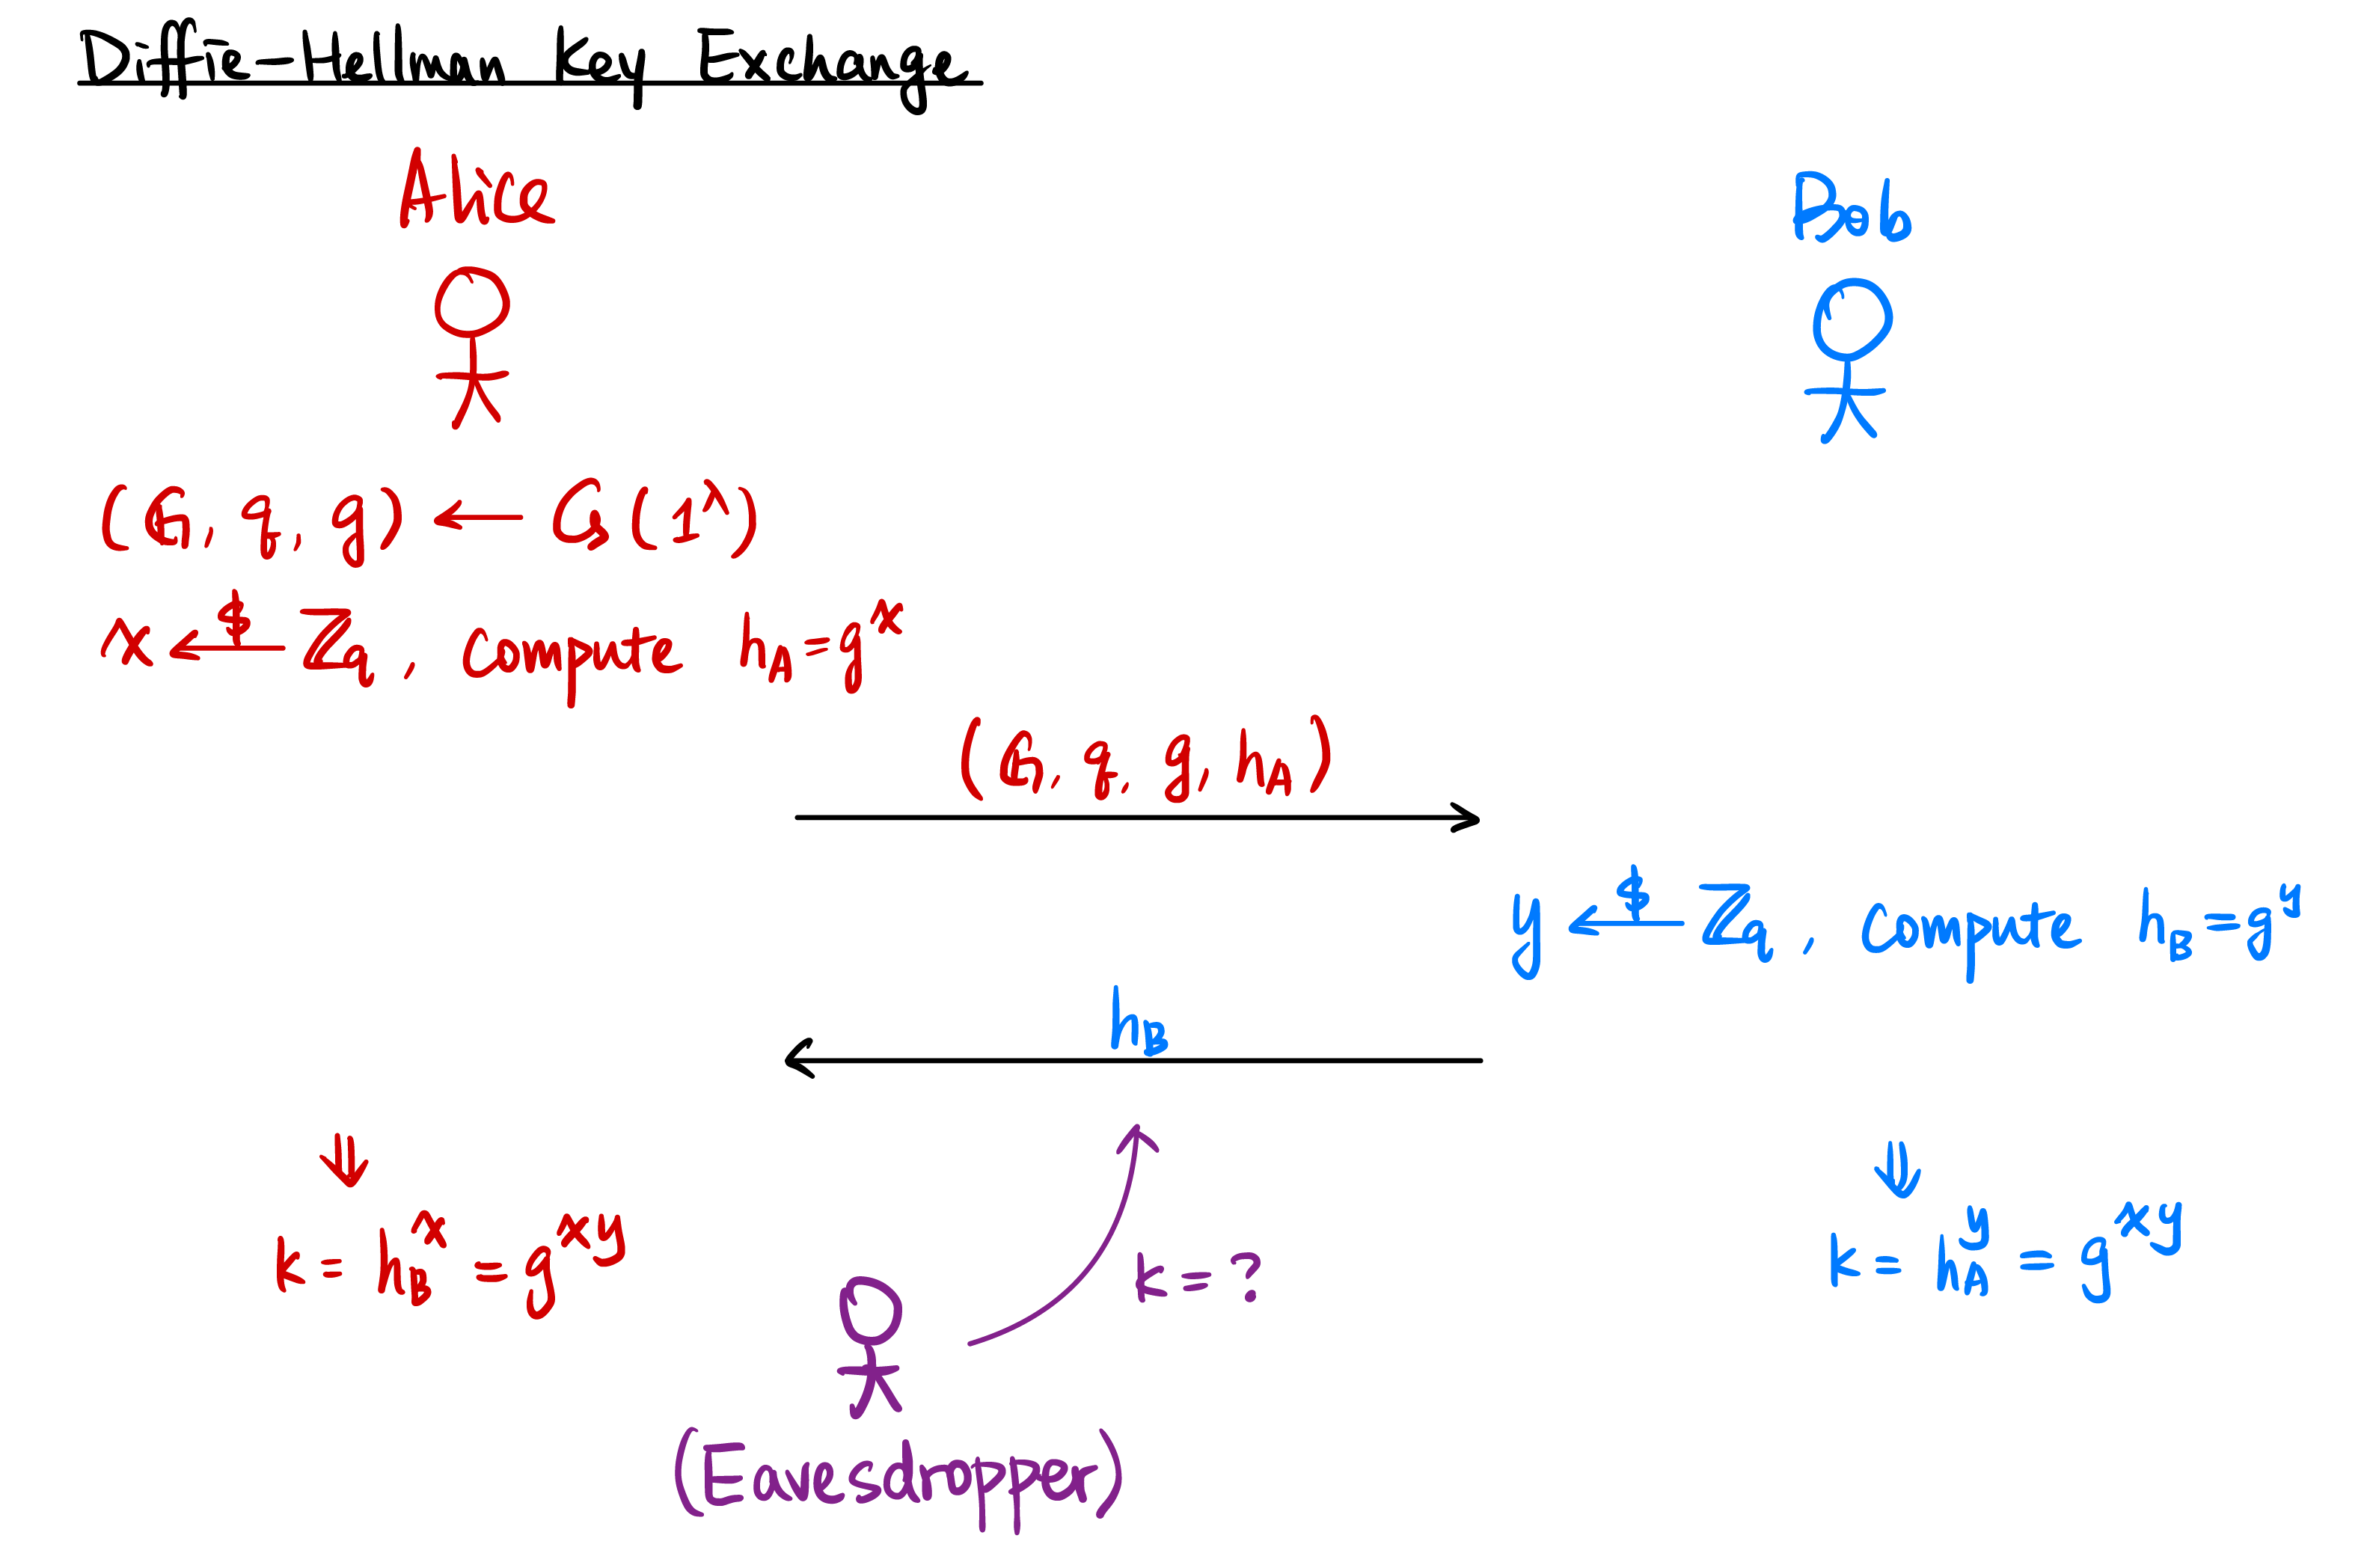
\includegraphics[width=0.8\textwidth]{images/2023-02-02/diffie-hellman.png}
\end{center}

What happens in practice is that parties run Diffie-Hellman key exchange to agree on a shared key. Using that shared key, they run symmetric-key encryption. This gives us efficiency. Additionally, private-key encryptions don't rely on heavy assumptions on the security of protocols (such as the DDH, RSA assumptions).

\subsection{Message Integrity}
Alice sends a message to Bob, how does Bob ensure that the message came from Alice?

\begin{center}
    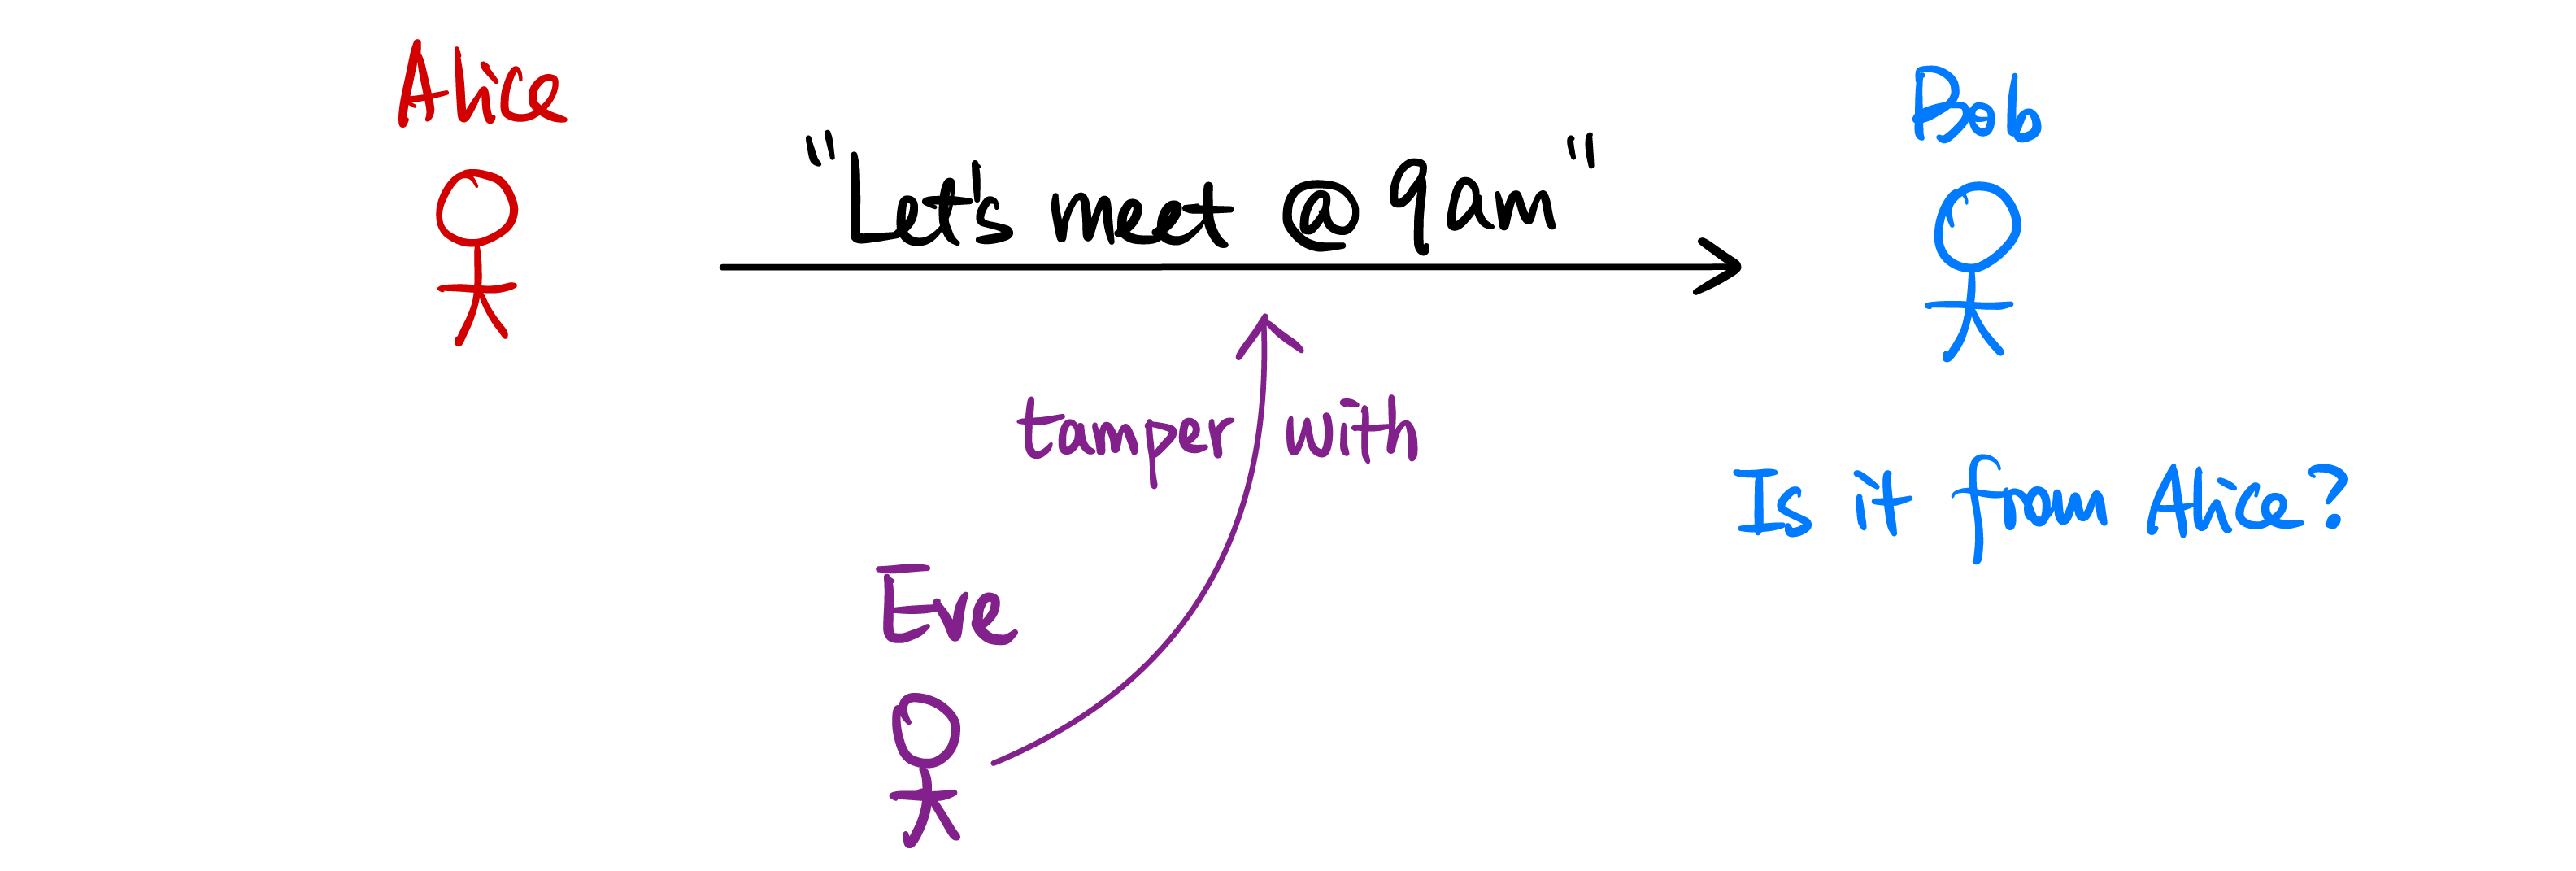
\includegraphics[width=0.8\textwidth]{images/2023-02-02/integrity.png}
\end{center}

We can build up another line of protocols to ensure message integrity. It's similar to encryption, but the parties run 2 algorithms: \emph{Authenticate} and \emph{Verify}.

Using a message $m$, Alice can generate a \emph{tag} or \emph{signature}, and Bob can verify $(m, t)$ is either valid or invalid.

Our adversary has been upgraded to an Eve who can now tamper with messages.

Similarly to encryption, we have symmetric-key and public-key encryption.

Using a shared key $k$, Alice can authenticate $m$ using $k$ to get a tag $k$. Similarly, Bob can verify whether $(m, t)$ is valid using $k$. This is called a Message Authentication Code.

\begin{center}
    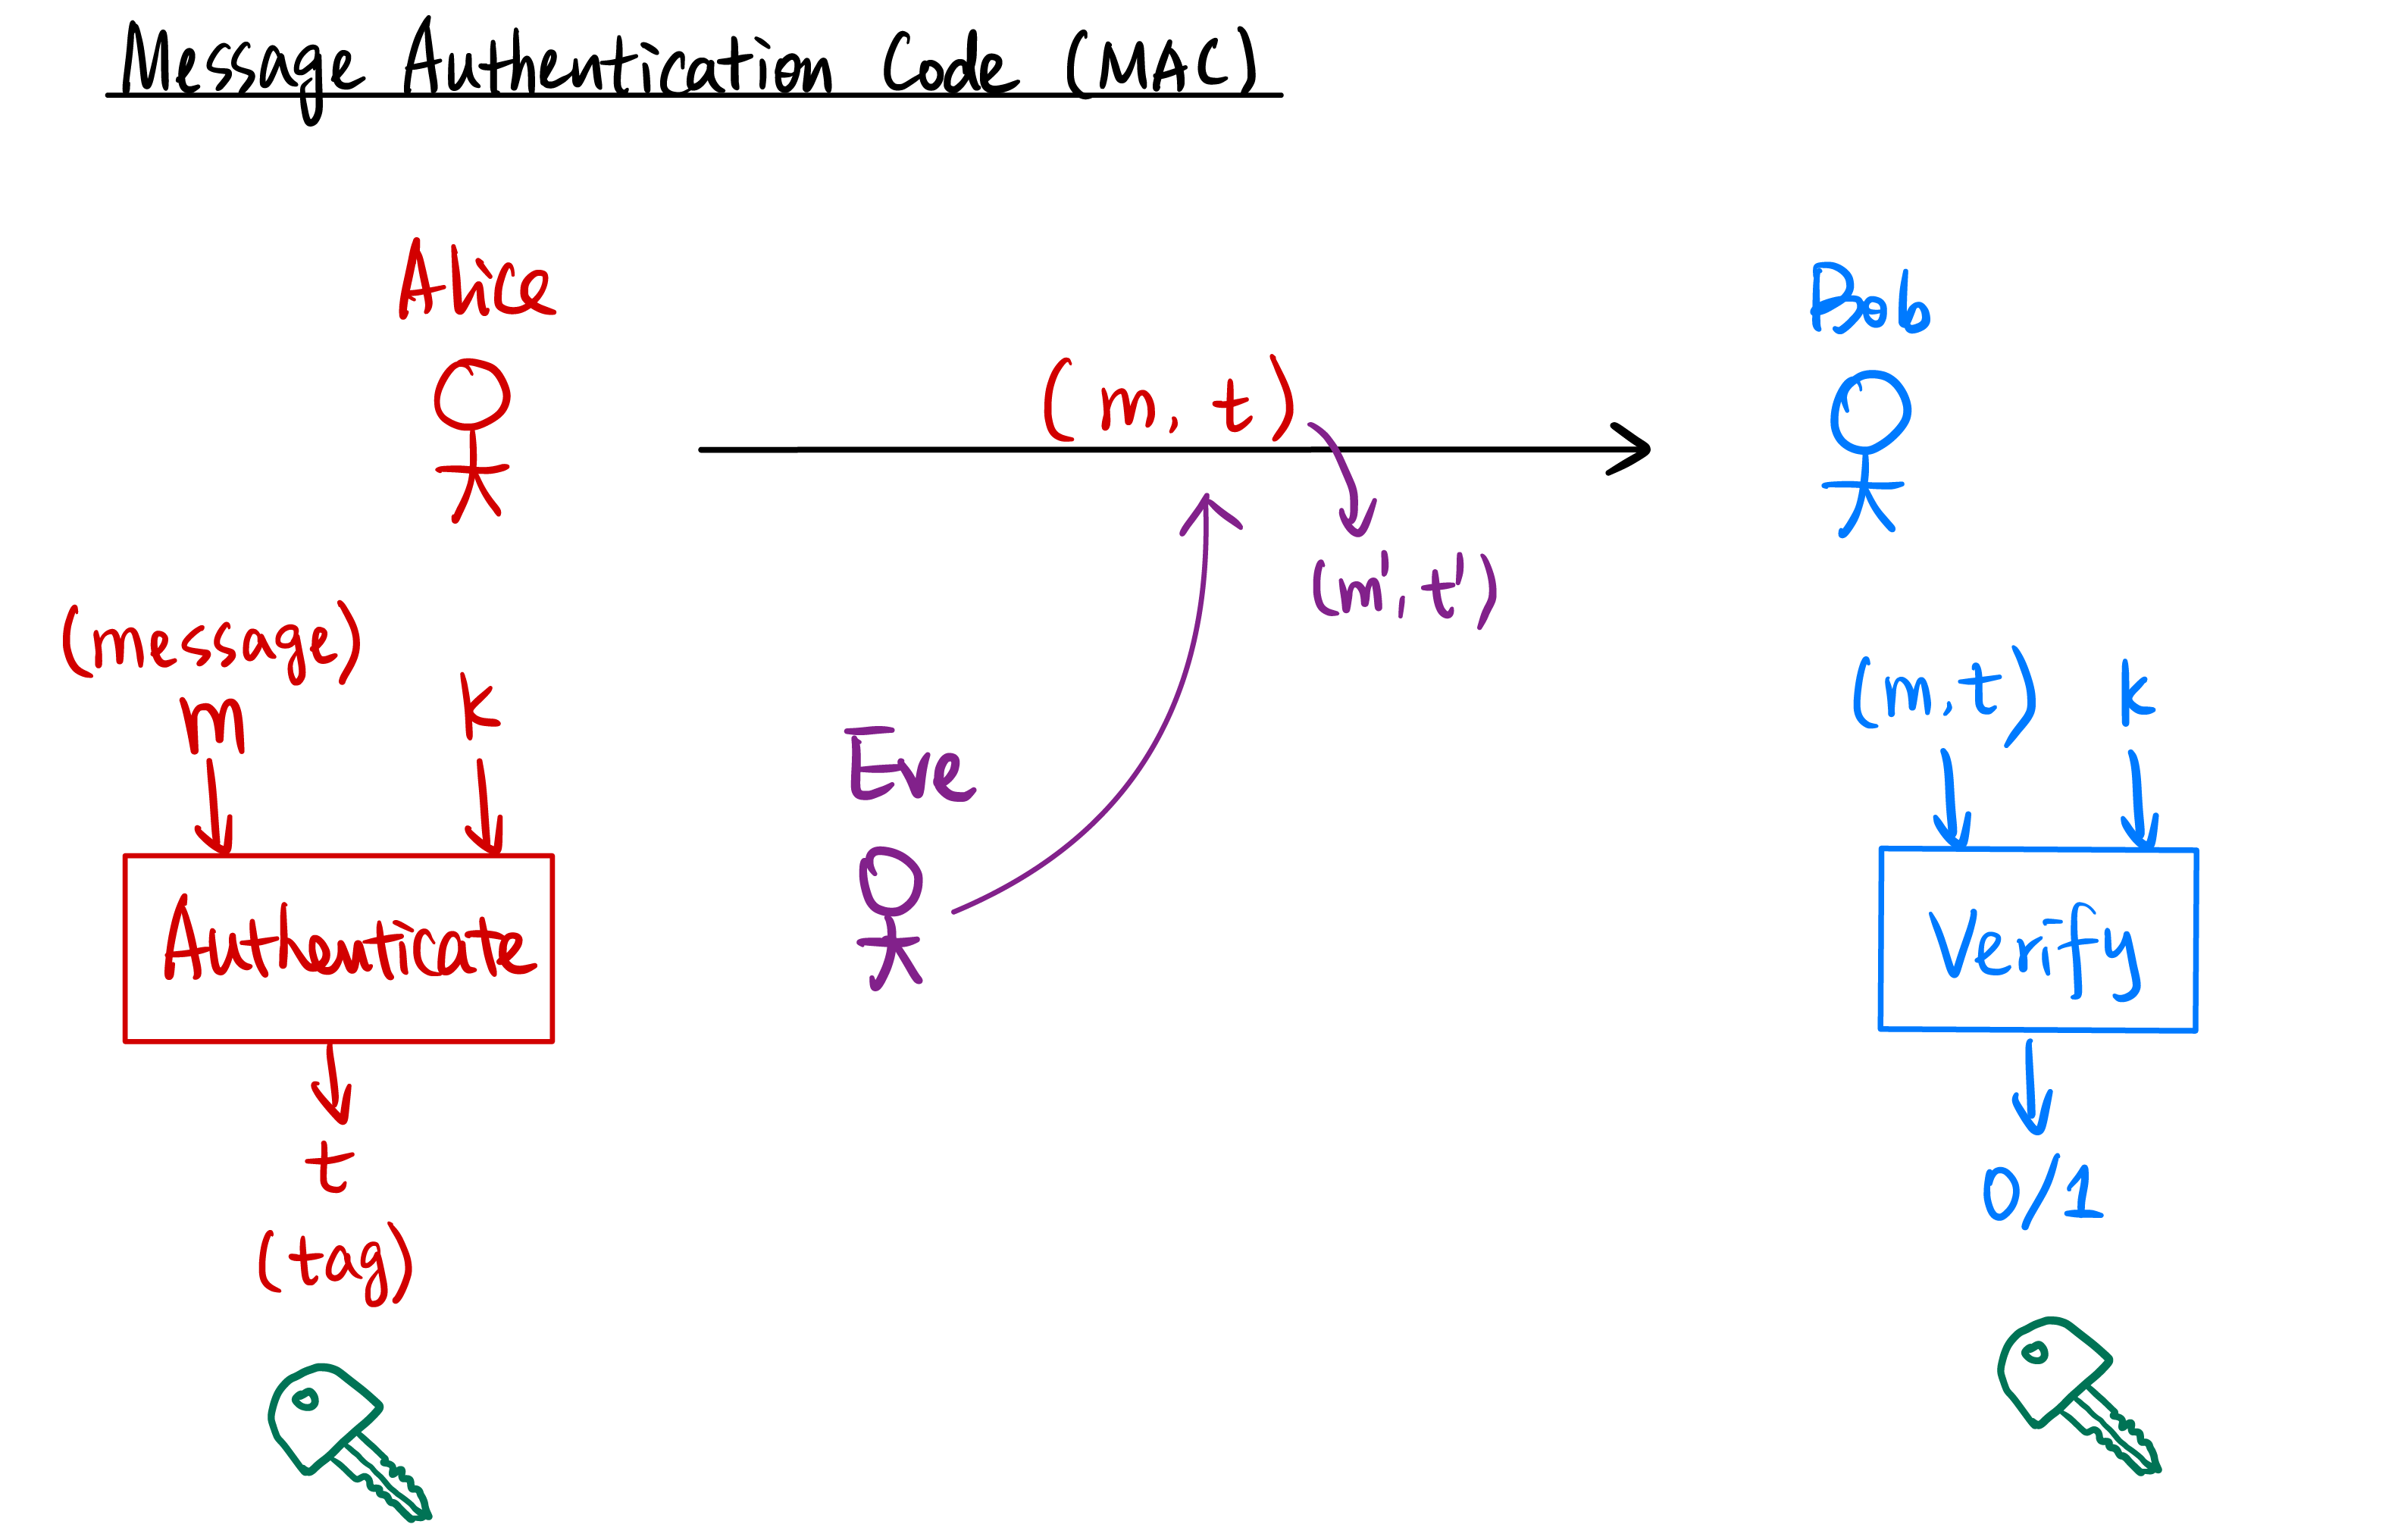
\includegraphics[width=0.8\textwidth]{images/2023-02-02/mac.png}
\end{center}

Using a public key $vk$ (verification key) and private key $sk$ (secret/signing key), Alice can sign a message $m$ using signing key $sk$ to get a \emph{signature} $\sigma$. Bob verifies $(m, \sigma)$ is valid using $vk$. This is called a Digital Signature.

\begin{center}
    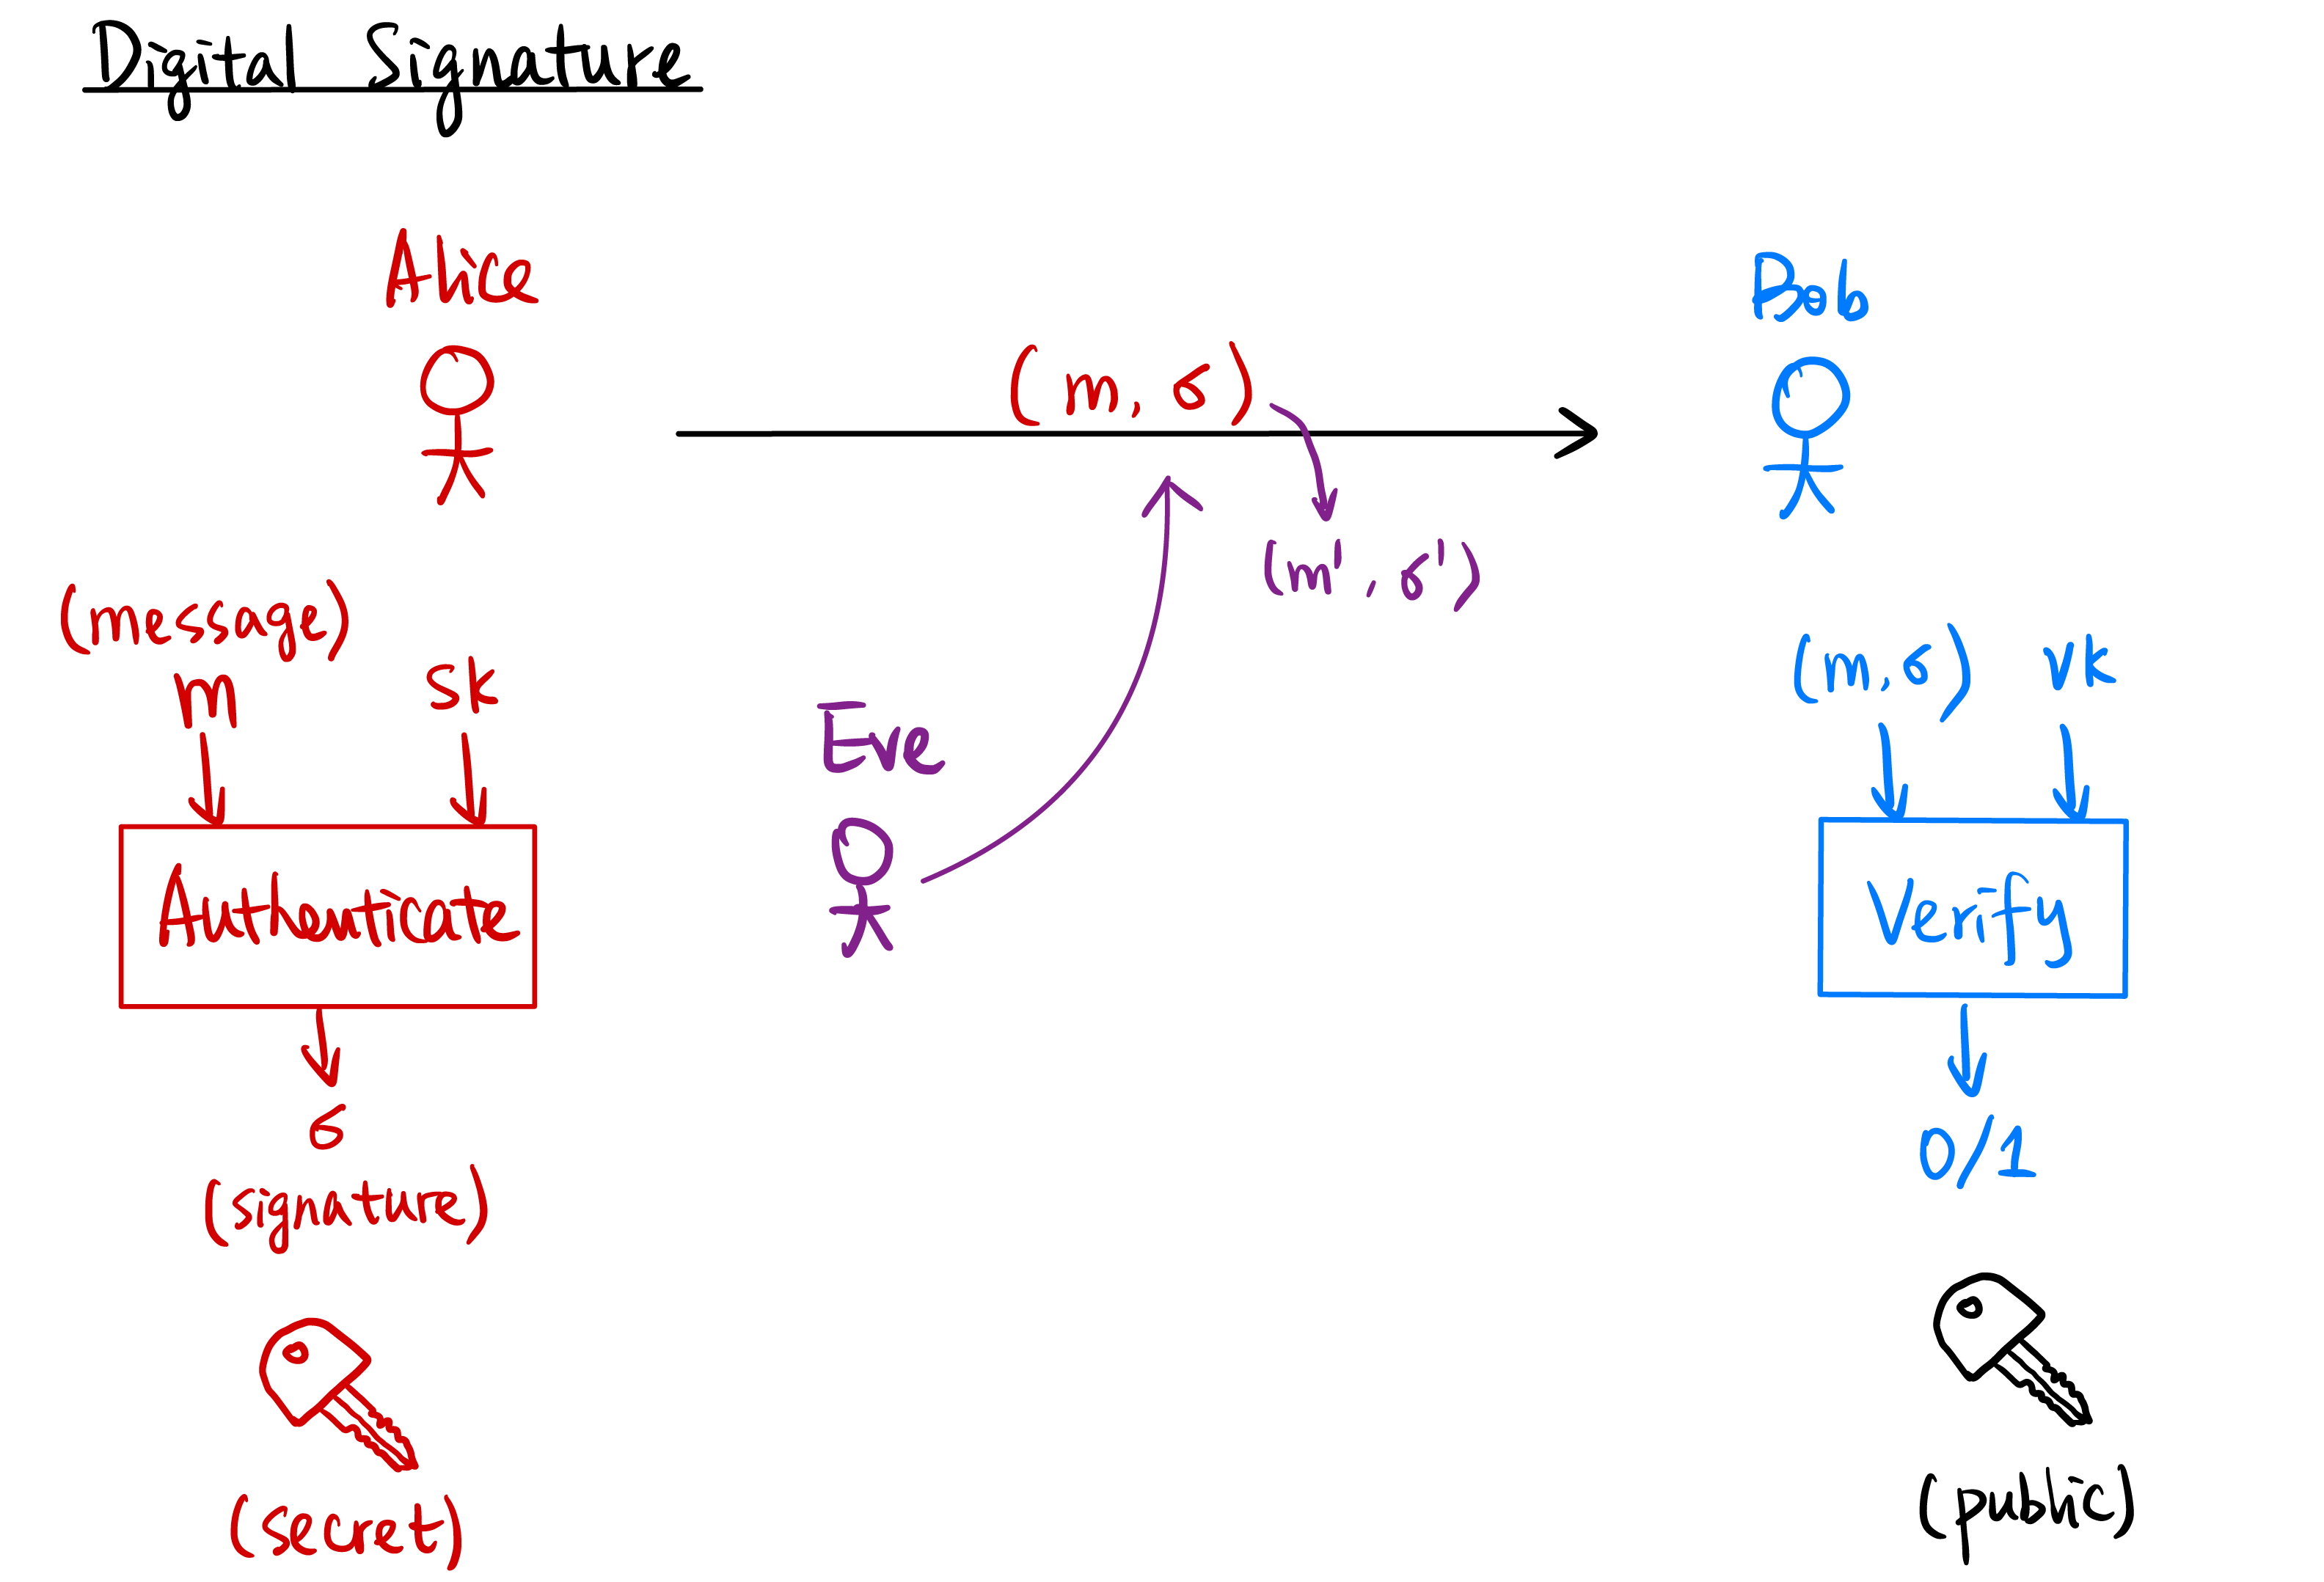
\includegraphics[width=0.8\textwidth]{images/2023-02-02/signature.png}
\end{center}

\subsubsection{Syntax}\label{sec:message-integrity:syntax}
The following is the syntax we use for MACs and digital signatures.

A message authentication code (MAC) scheme consists of $\Pi = (\Gen, \mathsf{Mac}, \mathsf{Verify})$.
\begin{description}
    \item[Generation.] $k\leftarrow \Gen(1^\lambda)$.
    \item[Authentication.] $t \leftarrow \mathsf{Mac}_k(m)$.
    \item[Verification] $0/1 := \mathsf{Verify}_k(m, t)$.
\end{description}

A digital signature scheme consists of $\Pi = (\Gen, \mathsf{Sign}, \mathsf{Verify})$.
\begin{description}
    \item[Generation.] $(sk, vk)\leftarrow \Gen(1^\lambda)$.
    \item[Authentication.] $\sigma \leftarrow \mathsf{Sign}_{sk}(m)$.
    \item[Verification] $0/1 := \mathsf{Verify}_{vk}(m, \sigma)$.
\end{description}

\subsubsection{Chosen-Message Attack}
Similar to chosen-plaintext attack from encryption, we have chosen-message attack security. An adversary chooses a number of messages to generate signatures or tags for. After that, the adversary will try to generate another valid pair of message and tag. We want to make sure that generating a new pair of message and tag is hard.

\begin{center}
    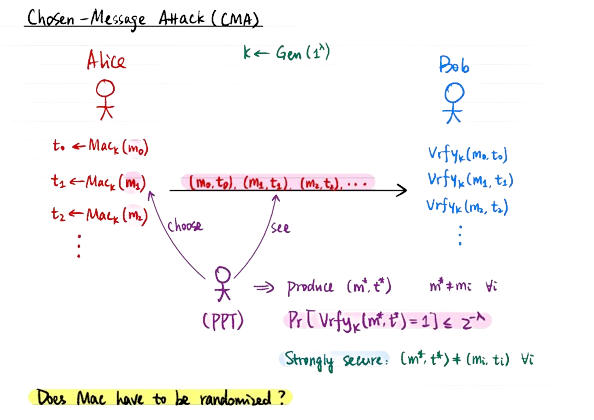
\includegraphics[width=0.8\textwidth]{images/2023-02-02/cma.png}
\end{center}

\subsubsection{Constructions}
Very briefly, we discuss constructions for MAC and digital signatures.

Using block ciphers, we have CBC-MAC. Using a hash function, we have HMAC.

For digital signatures, we have RSA which relies on the RSA assumption, or DSA which relies on discrete-log algorithms. There are also lattice signature schemes for post-quantum digital signatures.